\subsection{超新星} \label{transients.s1.sn}
超新星 (supernova; SN) は、星がその生涯の最期に爆発する現象であり、その爆発の実体として2つのシナリオが考えられている。
一方は、何らかの理由で白色矮星\footnote{恒星の場合、気体の圧力や核融合による輻射圧が重力とつりあって形状を保っており、白色矮星の場合は電子の縮退圧、中性子星の場合は中性子の縮退圧が、重力とつりあっている。}の質量が増大しチャンドラセカール質量\footnote{重力が電子の縮退圧を超える限界質量をチャンドラセカール質量とよび、それを超えた白色矮星は超新星爆発を起こす。}に達した時に、核暴走により白色矮星自体が爆発するというものである。
白色矮星質量を増大させる機構として、白色矮星と恒星の連星系において恒星のガスが白色矮星に降着するシナリオ、二つの白色矮星が重力波
放出を通し合体するシナリオが提案されている。
同様に白色矮星を起源とした核暴走として新星爆発が知られているが、この二つではその爆発の規模が大きく異なる。
新星爆発の場合は、白色矮星の表面上で一時的に核融合が暴走し爆発するだけで、白色矮星自体は爆発後も健在だが、超新星爆発の場合は白色矮星全体が爆発してしまい、後には何も残らず四散してしまうと考えられている。
もう一方のシナリオは、大質量星が自重を支えきれずに単独で重力崩壊し爆発するというものである。
大質量の恒星は内部に鉄などのコアをもつが、そのコアが重力崩壊を起こすと中心部に硬い原始中性子星がつくられ、それに衝突した物質がはね返って衝撃波をつくり爆発すると考えられている。% \citep[e.g.,][]{1994Natur.371..227N}。
このシナリオの超新星は、コアが重力崩壊することにちなんで、コア崩壊型超新星 (core-collapse supernova; CCSN) または重力崩壊型超新星とよばれる。
これらのシナリオは妥当なものだが、爆発に至る詳しいメカニズムはわかっておらず、コンピュータシミュレーションや観測事実の蓄積によって、その解明が試みられている。
超新星の分類は、歴史的にはスペクトルや光度曲線の特性によって行われ、\Figref{fig:transients.s1.sn}のように分類され命名されてきている。
連星系にある白色矮星の超新星爆発はIa型超新星に分類され、その他のIb型、Ic型、II型超新星はすべてコア崩壊型超新星である。
%例えばスペクトルに水素の吸収線が見られるものはII型に分類されるが、吸収線があるということは水素が豊富であることを示しており、\Figref{fig:transients.s1.sn}の右図のように水素が多く含まれた星が爆発したものと考えられる。
\begin{figure}[]
	\begin{minipage}{0.6\textwidth}
		\centering
		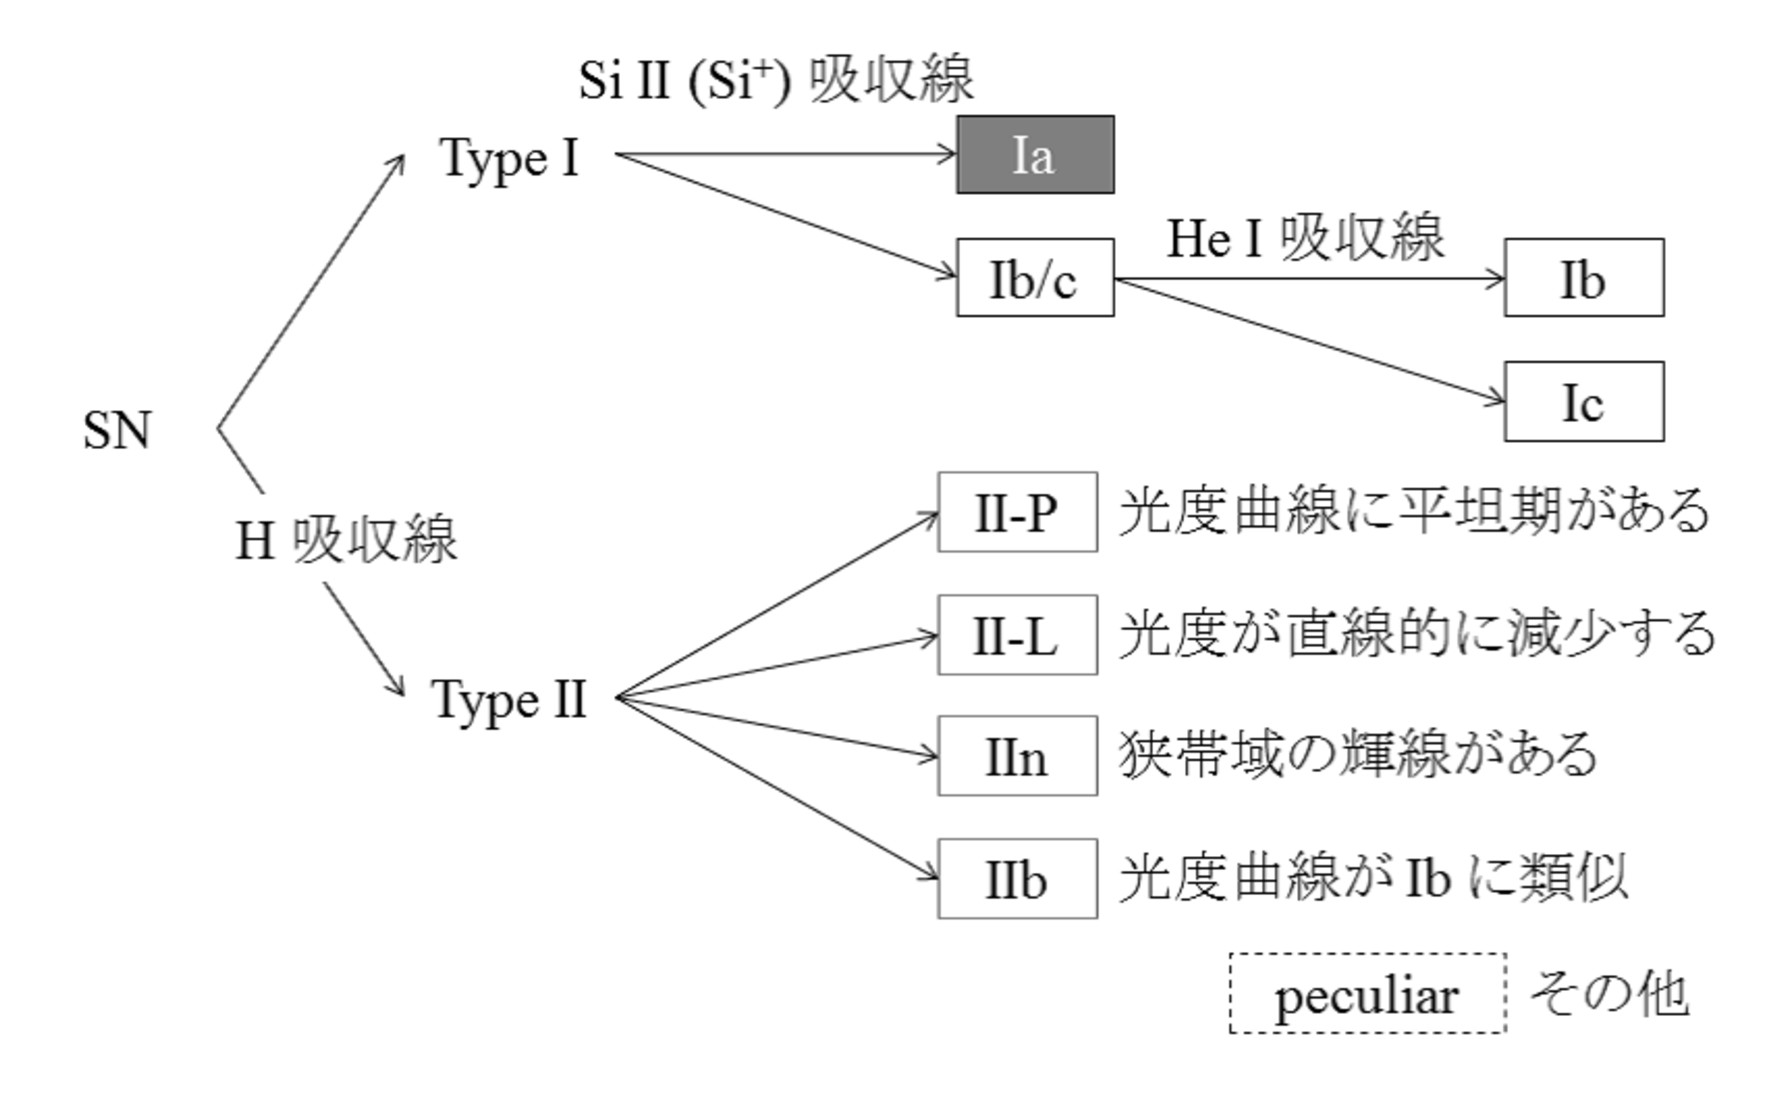
\includegraphics[width=\linewidth,clip]{transients/transients.s1.sn-class.eps}
	\end{minipage}
	\begin{minipage}{0.4\textwidth}
		\centering
		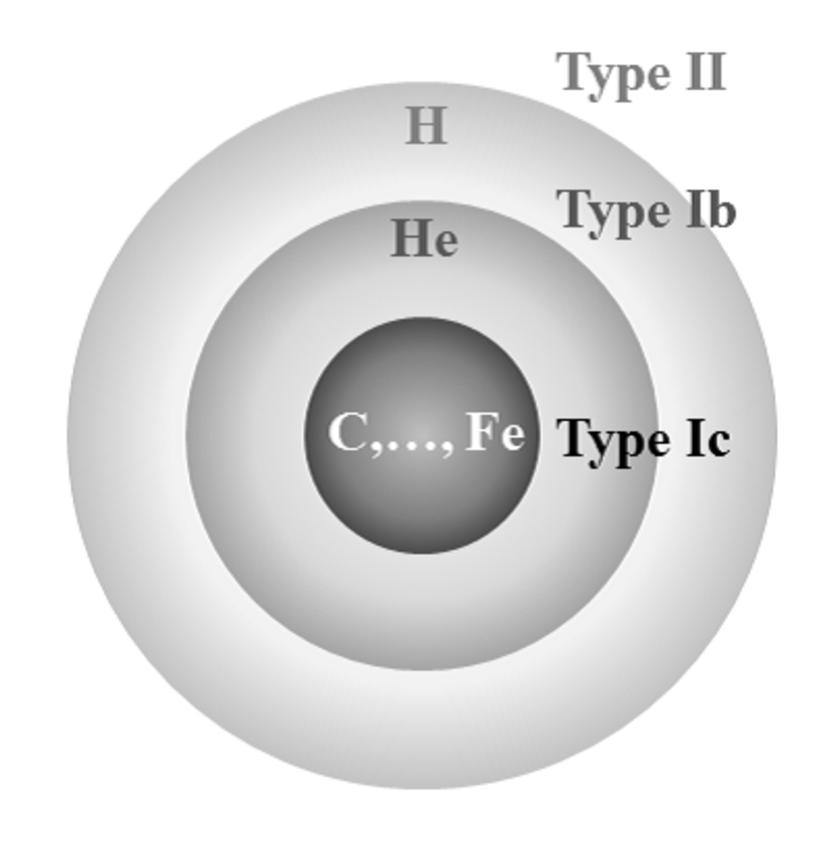
\includegraphics[width=0.7\linewidth,clip]{transients/transients.s1.ccsn.eps}
	\end{minipage}
	\caption{左図: 超新星の分類; 右図: コア崩壊型超新星となる以前の星の「たまねぎ構造」。}
	\label{fig:transients.s1.sn}
\end{figure}%

超新星爆発は主に光学望遠鏡によって発見され、電波望遠鏡で先んじて発見されたことはほとんどなかった。
%これは可視光域で明るいという理由の他に、光学望遠鏡は広い範囲を高い空間分解能で観測することに長けており、突発天体を発見しやすい装置であることも一因として挙げられる。
%またその探査では日本のアマチュア天文家による貢献も大きい。
%一方で従来の電波望遠鏡は、狭い範囲を極めて高い空間分解能で観測することに長けており\footnote{電波望遠鏡は、広い範囲を低い空間分解能で観測することにも長けている。}、それゆえ光学望遠鏡で発見された超新星を詳細に追観測することが主な役割だった。
SKAではこの状況を打破し、光学望遠鏡で発見された超新星の追観測のみならず、広い視野による広域探査によって電波帯域における超新星の発見を目指す。
また従来、Ia型超新星は暗すぎるために電波で検出されたことがないが \citep{2012ApJ...750..164C}、SKAによって初めてIa型超新星の電波観測が成功すると期待される。

超新星からの電波は、爆発の瞬間に放射されるのではなく、爆発前に星から噴出した物質に対して、爆発後に噴出した物質が衝突することによって放射されると考えられている。
したがって超新星を電波観測すると、爆発前後の星の状態を調べることができる。
また減光した後も、その噴出物は周りの星間物質と相互作用し続け、超新星残骸 (supernova remnant; SNR) とよばれる構造をなす。
その中では宇宙線の起源となる粒子加速が起こっていると考えられ、超新星残骸の電波観測によって他波長にわたる物理過程の解明が進むだろう。
可視光域で発見されている超新星のうち、従来の電波望遠鏡で観測できているものは一握りであるため、SKAによる高感度観測によって電波による観測サンプル数が増えれば、超新星の研究にとって大きなブレイクスルーとなるに違いない。
